\documentclass[10pt,twocolumn]{article}

% ── Packages ──
\usepackage[margin=0.75in]{geometry}
\usepackage{times}
\usepackage{amsmath,amssymb}
\usepackage{booktabs}
\usepackage{graphicx}
\usepackage[hypertexnames=false]{hyperref}
\usepackage{xcolor}
\usepackage{caption}
\usepackage{subcaption}
\usepackage{enumitem}
\usepackage{microtype}
\usepackage{float}
\usepackage{pgfplots}
\usepackage{authblk}
\pgfplotsset{compat=1.18}
\usepgfplotslibrary{groupplots}
\usetikzlibrary{patterns}

% ── Float placement ──
\setcounter{topnumber}{2}
\setcounter{bottomnumber}{2}
\setcounter{totalnumber}{4}
\renewcommand{\topfraction}{0.9}
\renewcommand{\bottomfraction}{0.8}
\renewcommand{\textfraction}{0.07}
\renewcommand{\floatpagefraction}{0.85}
\renewcommand{\dbltopfraction}{0.9}
\renewcommand{\dblfloatpagefraction}{0.85}
\setlength{\textfloatsep}{8pt plus 2pt minus 2pt}
\setlength{\floatsep}{6pt plus 2pt minus 2pt}
\setlength{\intextsep}{6pt plus 2pt minus 2pt}

% ── Colors ──
\definecolor{fiblue}{HTML}{2171B5}
\definecolor{triorange}{HTML}{E6550D}
\definecolor{reconred}{HTML}{CB181D}
\definecolor{attnblue}{HTML}{6BAED6}
\definecolor{predgreen}{HTML}{31A354}
\definecolor{measred}{HTML}{DE2D26}
\pgfplotsset{
  every axis/.append style={
    label style={font=\small},
    tick label style={font=\footnotesize},
    legend style={font=\footnotesize, legend cell align=left},
  },
}

% ── Formatting ──
\setlength{\parskip}{0.4em}
\setlength{\parindent}{0em}

\title{%
  \textbf{The Hidden Bottleneck in MLA Serving:}\\
  \textbf{Reconstruction GEMMs, INT4 Quantization, and the L2 Cache Barrier}
}

\author[1]{Robert Zhang} % Link author to affiliation [1]
\affil[1]{Purdue University} % Define affiliation [1]
\affil[1]{\texttt{zhan4808@purdue.edu}} % Add email to the same affiliation bloc
\date{}

\begin{document}
\maketitle

% ══════════════════════════════════════════════════════════════════════════════
\begin{abstract}
Multi-head Latent Attention (MLA) compresses KV cache via low-rank latent projections, greatly reducing memory traffic for the attention kernel.  We show that this compression creates a \emph{new} dominant bottleneck: the \textbf{reconstruction GEMMs}, weight-absorbed batch matrix multiplications that recover full-dimensional K/V from compressed latents, consume \textbf{61\% of attention-layer time} at batch size~1 on DeepSeek-V3-scale architectures (128~heads, 61~layers), exceeding the attention kernel itself.  These BMMs are memory-bound at all practical batch sizes (arithmetic intensity 1--93 vs.\ H100 roofline crossover at~295).

We investigate INT4 weight-only quantization as a mitigation.  Selective INT4 of reconstruction weights preserves quality ($\Delta$PPL~=~+0.051 on wikitext-2, vs.\ +6.057 for naive whole-model INT4).  However, a custom batched W4A16 Triton kernel achieves only 0.49$\times$ of cuBLAS FP16; we identify \textbf{two stacked root causes}.  First, \emph{partial L2 residency}: warm-state hardware counters (\texttt{ncu --cache-control none}) show ${\sim}75\%$ of the 16~MB reconstruction weight matrix is served from L2 in steady state, at an effective 3.5--4.6~TB/s, weakening the HBM-bound roofline assumption that motivates quantization.  The effective residency capacity is ${\sim}36$~MB --- measured DRAM re-reads collapse at 16--32~MB and snap to 100\% at $\geq$40~MB --- below the nominal 50~MB L2.  Second, \emph{dequantization compute}: a fixed-shape weight-rotation intervention that forces FP16 weights out of L2 shows INT4 \emph{still} loses (1.12$\times$ slower), because the W4A16 kernel is SM-bound from dequantization (up to 79\% SM utilization) and runs 2.7$\times$ above its memory entitlement.  L2 residency removes most of the theoretical INT4 upside; dequantization overhead destroys the rest.  Scaling weight size from 8~MB to 128~MB, the kernel-level INT4/FP16 gap drops from 1.9$\times$ to parity ($\sim$1.1$\times$) --- INT4 never wins.  We are not aware of prior published characterization of this failure mode.

We validate our profiling methodology through an independent FlashInfer vs.\ Triton kernel comparison on Llama-3-8B, reproducing known results (89\% vs.\ 80\% HBM utilization in decode; 2.6$\times$ prefill gap from TMA hardware loads) and contributing new NCU-level root cause analysis.  All code and data are publicly available.
\end{abstract}

% ══════════════════════════════════════════════════════════════════════════════
\section{Introduction}

Multi-head Latent Attention (MLA)~\cite{deepseekv2} compresses the KV cache through low-rank latent projections, achieving a 7.1$\times$ reduction in KV memory traffic and powering frontier models including DeepSeek-V2 and V3~\cite{deepseekv3}.  But this compression requires full-dimensional K and V to be \emph{reconstructed} from compressed latents at inference time via weight-absorbed batch matrix multiplications (BMMs).  Prior work has focused on MLA's memory savings; the runtime cost of reconstruction has not been studied.

We show that this cost is the \textbf{dominant bottleneck} in MLA attention layers.  On DeepSeek-V3-scale architectures (128 heads, 61 layers), reconstruction GEMMs consume 61\% of per-layer time at batch size~1, exceeding the attention kernel itself.  This overhead is fixed per query, independent of KV length, and invisible to standard attention benchmarks.  MLA's compression, in other words, shifts the bottleneck from KV cache reads to weight-matrix reads for reconstruction.

Since reconstruction is memory-bound (arithmetic intensity 1--93 vs.\ H100 roofline crossover at~295), INT4 weight-only quantization is a natural mitigation.  Selective INT4 preserves quality ($\Delta$PPL~=~+0.051), but a custom Triton W4A16 kernel achieves only 0.49$\times$ of cuBLAS FP16, far from the 3.9$\times$ predicted by roofline.  We trace this to what we term the \textbf{L2 cache barrier} \emph{combined with a dequantization-bound kernel}: warm-state counters show ${\sim}75\%$ of the 16~MB reconstruction weight matrix is served from L2 (effective 3.5--4.6~TB/s) rather than HBM at 3.35~TB/s, so reducing precision saves HBM bandwidth that was largely not the bottleneck (Figure~\ref{fig:l2barrier}); and even when residency is experimentally removed, the W4A16 kernel's dequantization compute keeps it at or below FP16 parity.  Scaling weight size across the L2 boundary, the INT4/FP16 time ratio drops from 1.9$\times$ at 8~MB toward parity at 128~MB, with the transition at 32--40~MB --- the \emph{effective} residency capacity, below the nominal 50~MB (Figure~\ref{fig:l2sweep}).  MLA's compression paradoxically makes reconstruction weights \emph{too small} to benefit from weight-only quantization.

We validate our profiling methodology through an independent FlashInfer~\cite{flashinfer} vs.\ Triton~\cite{triton} kernel comparison on Llama-3-8B (Section~\ref{sec:validation}), reproducing known performance gaps and contributing new NCU-level root cause analysis.

\textbf{Contributions:}
\begin{itemize}[leftmargin=*,topsep=0pt]
  \item \textbf{Reconstruction GEMM overhead}: first quantification showing 61\% of MLA attention-layer time at bs=1 (2.17~ms/token across 61~layers).
  \item \textbf{The L2 cache barrier}: roofline-predicted 3.9$\times$ INT4 speedup collapses to 0.49$\times$ through two stacked mechanisms --- partial L2 residency of the weights (75\% L2-served; effective capacity ${\sim}36$~MB, effective serving bandwidth 3.5--4.6~TB/s) and a dequantization-bound INT4 kernel that loses to FP16 even when residency is experimentally removed.  Validated by a weight-size sweep, warm-state counter analysis (\texttt{--cache-control none}), and a fixed-shape weight-rotation intervention.  We are not aware of prior published characterization of this failure mode.
  \item \textbf{Selective INT4 quality}: reconstruction weights tolerate INT4 well (+0.051 PPL), establishing them as targets once kernel support matures.
  \item \textbf{NCU-level kernel analysis}: TMA vs.\ global-load root cause, corrected L1 metrics on Hopper, and the occupancy paradox (fewer warps, more bandwidth).
\end{itemize}

% ══════════════════════════════════════════════════════════════════════════════
\section{Experimental Setup}

\subsection{Hardware}
Primary measurements use a single NVIDIA H100 80GB SXM5 (HBM3).  Cross-hardware validation uses a single NVIDIA A100 80GB SXM4 (HBM2e).  Reference peaks for H100: 3.35~TB/s HBM bandwidth, 989.4~TFLOPS BF16 tensor core, 132 SMs, 50~MB L2 cache.  Reference peaks for A100: 2.0~TB/s HBM bandwidth, 312~TFLOPS BF16 tensor core, 108 SMs, 40~MB L2 cache.  GPU clocks were not locked on either platform (\texttt{nvidia-smi -lgc}); Section~\ref{sec:repro} quantifies the resulting variance.

\subsection{Software}
SGLang (commit \texttt{7ef18be}), PyTorch 2.9.1+cu128, FlashInfer 0.6.6, Triton 3.5.1, CUDA 12.8, NCU 2025.1.1.

\subsection{Model Configurations}

\begin{table}[h]
\centering
\small
\caption{Configurations used in this work.  DS-V3 shapes ($H{=}128$, $d_\text{lora}{=}512$) are synthetic microbenchmark dimensions only (no weights loaded).  DS-V2-Lite is used for perplexity evaluation; Qwen2.5-7B for end-to-end decomposition.}
\label{tab:configs}
\begin{tabular}{@{}lccccc@{}}
\toprule
Model & $H_q$ & $H_{kv}$ & $d$ & Type & KV LoRA \\
\midrule
Llama-3-8B        & 32  & 8   & 128 & GQA 4:1 & ---  \\
DS-V3 shapes      & 128 & 128 & 128 & MLA     & 512  \\
DS-V2-Lite (15.7B) & 16 & 16  & 128 & MLA     & 512  \\
Qwen2.5-7B        & 28  & 4   & 128 & GQA 7:1 & ---  \\
\bottomrule
\end{tabular}
\end{table}

\textbf{Model choice rationale.}  Llama-3-8B is the standard FlashInfer/Triton benchmark target.  DeepSeek-V3 shapes ($H{=}128$, $d_\text{lora}{=}512$) define the MLA microbenchmarks: the full model is 671B and requires multi-GPU serving, so we instantiate its BMM dimensions directly without loading weights.  DS-V2-Lite (15.7B, same MLA architecture) is the smallest single-GPU MLA model available, used for perplexity evaluation.  Qwen2.5-7B provides the GQA end-to-end baseline.

\subsection{Methodology}

\textbf{Timing.}  CUDA events with 10+ warmup iterations, median of 100+ timed iterations.  Reproducibility verified across 3 independent trials (Section~\ref{sec:repro}).

\textbf{FLOP counting.}  Standard attention: $4 \cdot B \cdot \frac{S^2}{2} \cdot H \cdot d$ (QK$^\top$ matmul + AV matmul, $\times 2$ for multiply-accumulate, $\div 2$ for causal masking).  Reconstruction uses $M \times K \times N \times 2$ per BMM per head.

\textbf{Bandwidth formula.}  Decode: $\text{BW} = (\text{KV}_\text{read} + Q_\text{read} + O_\text{write}) / t_\text{median}$, where KV accounts for 99.8\% of bytes.

\textbf{NCU profiling.}  Collected with \texttt{ncu --set full --profile-from-start no} (kernel replay); overhead excluded from bandwidth runs.  \textbf{Cache-state caveat:} kernel replay defaults to \texttt{--cache-control all}, which flushes GPU caches before every measured launch.  All replay-based counters in this paper are therefore \emph{cold-cache} measurements; they are valid for kernel classification (DRAM- vs.\ SM-bound) but carry no information about steady-state cache residency.  Residency claims are based exclusively on (a) warm-loop counters collected with \texttt{--cache-control none} and (b) timing-only interventions (Section~\ref{sec:l2barrier}).

\textbf{Timing floor.}  Per-launch CUDA-event measurement of these microsecond-scale kernels carries a ${\sim}15.5~\mu$s launch/eventing floor on our stack (a 0.5~MB bmm times identically to a 16~MB one).  Where kernel-level conclusions are required we therefore also report CUDA-graph timing (20+ launches captured per graph, median of 50 replays), which removes per-launch CPU overhead.

\begin{table}[h]
\centering
\small
\caption{NCU metrics collected and their interpretation.}
\label{tab:ncu_metrics}
\begin{tabular}{@{}ll@{}}
\toprule
Metric & Interpretation \\
\midrule
\texttt{dram\_\_throughput}             & HBM utilization (\% peak) \\
\texttt{sm\_\_throughput}               & SM utilization (\% peak) \\
\texttt{sm\_\_warps\_active}            & Active warp occupancy \\
L1/L2 sector hit/miss counts           & Cache hierarchy behavior \\
\texttt{launch\_\_registers\_per\_thread} & Register pressure \\
\texttt{smsp\_\_inst\_executed\_pipe\_tensor} & Tensor core instruction count \\
\bottomrule
\end{tabular}
\end{table}

% ══════════════════════════════════════════════════════════════════════════════
\section{Attention Kernel Validation}
\label{sec:validation}

Before presenting our MLA findings, we validate the profiling methodology by comparing FlashInfer and Triton attention kernels on Llama-3-8B, a well-studied GQA configuration.  This reproduces known performance gaps and establishes the measurement infrastructure used in subsequent sections.

\subsection{Decode: Bandwidth Scaling}
\label{sec:decode}

\begin{table}[h]
\centering
\small
\caption{Decode performance, Llama-3-8B GQA, $L_{kv}=2048$.}
\label{tab:decode_bs}
\begin{tabular}{@{}rrrrrr@{}}
\toprule
BS & FI (ms) & Tri (ms) & FI BW & Tri BW & Speedup \\
\midrule
  1 & 0.028 & 0.057 &  298 &  147 & \textbf{2.03$\times$} \\
  4 & 0.032 & 0.058 & 1056 &  582 & 1.82$\times$ \\
 16 & 0.058 & 0.070 & 2317 & 1910 & 1.21$\times$ \\
 64 & 0.187 & 0.218 & 2870 & 2470 & 1.16$\times$ \\
128 & 0.364 & 0.416 & 2957 & 2585 & 1.14$\times$ \\
256 & 0.720 & 0.806 & \textbf{2987} & \textbf{2669} & 1.12$\times$ \\
\bottomrule
\end{tabular}
\end{table}

Both backends are firmly memory-bound (Table~\ref{tab:decode_bs}).  FlashInfer peaks at 2,987~GB/s (89\% of 3.35~TB/s) while Triton peaks at 2,669~GB/s (80\%).  The gap narrows from 2$\times$ at bs=1 (launch-overhead dominated) to 1.12$\times$ at bs=256 (bandwidth-saturated); Figure~\ref{fig:decode_bw} shows the full scaling curve.

\begin{figure}[t]
\centering
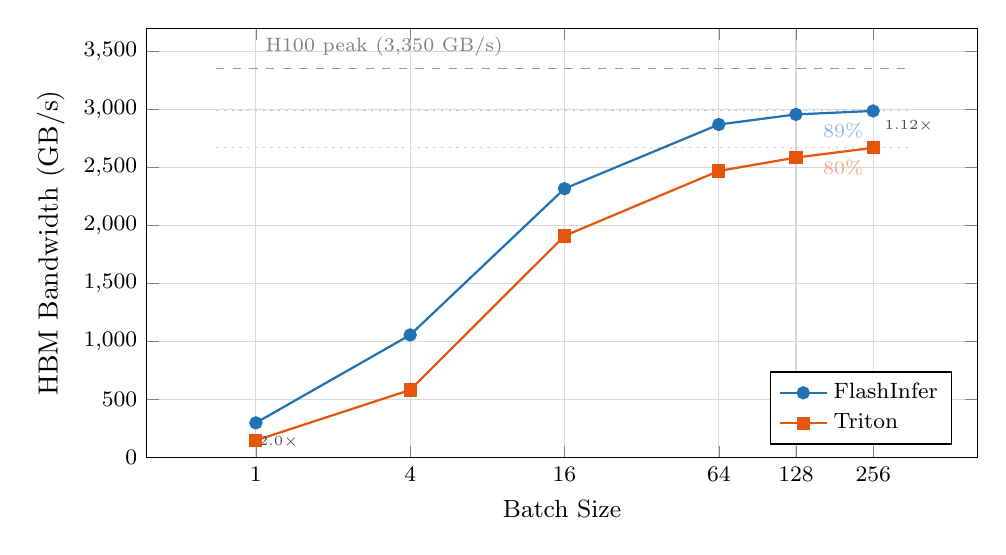
\begin{tikzpicture}
\begin{axis}[
  width=\columnwidth,
  height=0.58\columnwidth,
  xlabel={Batch Size},
  ylabel={HBM Bandwidth (GB/s)},
  xmode=log, log basis x=2,
  xtick={1,4,16,64,128,256},
  xticklabels={1,4,16,64,128,256},
  ymin=0, ymax=3700,
  ytick={0,500,1000,1500,2000,2500,3000,3500},
  grid=major, grid style={gray!30},
  every axis plot/.append style={thick},
  ylabel near ticks,
  clip=false,
  legend style={at={(0.97,0.03)}, anchor=south east},
]
% H100 peak
\addplot[dashed, black!40, thin, forget plot]
  coordinates {(0.7,3350) (350,3350)};
\node[font=\scriptsize, black!50, anchor=south west]
  at (axis cs:1,3370) {H100 peak (3{,}350 GB/s)};
% 89% line
\addplot[dotted, fiblue!40, thin, forget plot]
  coordinates {(0.7,2987) (350,2987)};
\node[font=\scriptsize, fiblue!50, anchor=north east]
  at (axis cs:256,2970) {89\%};
% 80% line
\addplot[dotted, triorange!40, thin, forget plot]
  coordinates {(0.7,2669) (350,2669)};
\node[font=\scriptsize, triorange!50, anchor=north east]
  at (axis cs:256,2650) {80\%};
% FlashInfer
\addplot[fiblue, mark=*, mark size=2] coordinates {
  (1,298) (4,1056) (16,2317) (64,2870) (128,2957) (256,2987)
};
% Triton
\addplot[triorange, mark=square*, mark size=2] coordinates {
  (1,147) (4,582) (16,1910) (64,2470) (128,2585) (256,2669)
};
% Speedup annotations
\node[font=\tiny, black!70, anchor=north east] at (axis cs:1.6,270) {2.0$\times$};
\node[font=\tiny, black!70, anchor=north west] at (axis cs:260,2987) {1.12$\times$};
\legend{FlashInfer, Triton}
\end{axis}
\end{tikzpicture}
\caption{Decode bandwidth vs.\ batch size (Llama-3-8B, $L_{kv}{=}2048$).  Both backends approach HBM saturation; FlashInfer peaks at 89\% of H100 peak.  The gap narrows from 2$\times$ at bs=1 to 1.12$\times$ at bs=256 as launch overhead becomes negligible relative to streaming KV reads.}
\label{fig:decode_bw}
\end{figure}

\begin{table}[h]
\centering
\small
\caption{Decode performance, Llama-3-8B GQA, bs=64, varying $L_{kv}$.}
\label{tab:decode_kv}
\begin{tabular}{@{}rrrrrr@{}}
\toprule
$L_{kv}$ & FI (ms) & Tri (ms) & FI BW & Tri BW & Speedup \\
\midrule
  256 & 0.037 & 0.065 & 1859 & 1053 & \textbf{1.76$\times$} \\
  512 & 0.059 & 0.069 & 2273 & 1950 & 1.17$\times$ \\
 1024 & 0.102 & 0.113 & 2648 & 2389 & 1.11$\times$ \\
 2048 & 0.187 & 0.217 & 2875 & 2476 & 1.16$\times$ \\
 4096 & 0.360 & 0.409 & 2984 & 2624 & 1.14$\times$ \\
 8192 & 0.716 & 0.790 & \textbf{3000} & \textbf{2720} & 1.10$\times$ \\
\bottomrule
\end{tabular}
\end{table}

FlashInfer approaches 3,000~GB/s at $L_{kv}=8192$, saturating HBM at 89.6\% of peak (Table~\ref{tab:decode_kv}).

\subsection{Decode: NCU Analysis}

\begin{table}[h]
\centering
\small
\caption{NCU metrics, decode, bs=64, $L_{kv}=2048$.}
\label{tab:ncu_decode}
\begin{tabular}{@{}lcc@{}}
\toprule
Metric & FlashInfer & Triton (Stage 1) \\
\midrule
Kernel       & \texttt{BatchPrefill..} & \texttt{\_fwd\_grouped..} \\
DRAM util.   & \textbf{84\%} & 76\% \\
SM util.     & 17\% & 28\% \\
Regs/thread  & \textbf{183} & 76 \\
Active warps & 12.2\% & \textbf{35.4\%} \\
Tensor insts & 2.16M & 2.10M \\
L2 hit rate  & 0.4\% & 1.0\% \\
Duration     & \textbf{191~$\mu$s} & 217~$\mu$s \\
\bottomrule
\end{tabular}
\end{table}

\textbf{The occupancy paradox.}  Table~\ref{tab:ncu_decode} shows FlashInfer uses 183 registers/thread (2.4$\times$ Triton's 76), yielding only 12.2\% active warps vs.\ 35.4\%.  Yet FlashInfer achieves 84\% DRAM throughput vs.\ 76\%.  This shows that \emph{memory access pattern quality dominates occupancy} for bandwidth-bound kernels: FlashInfer's fused design with coalesced, pipelined accesses extracts more bandwidth per warp than Triton's higher-occupancy two-phase approach.

\textbf{Two-phase overhead.}  Triton splits attention into Stage~1 (KV scatter-gather, 217~$\mu$s) and Stage~2 (softmax reduction, 10~$\mu$s).  Stage~2 adds 4.4\% overhead but achieves 73.8\% occupancy with only 30 registers, a well-optimized reduction kernel.

\textbf{L2 irrelevance at scale.}  Both backends show $<$1\% L2 hit rate.  The KV cache at bs=64 is $64 \times 2048 \times 8 \times 128 \times 2 = 256$~MB, far exceeding the 50~MB L2.  GQA's 4:1 head sharing provides no cache benefit at this scale.

\subsection{Prefill: TFLOPS Scaling}
\label{sec:prefill}

\begin{table}[h]
\centering
\small
\caption{Prefill performance, Llama-3-8B GQA.  TFLOPS uses corrected formula ($4 B S^2 H d / 2$).}
\label{tab:prefill}
\begin{tabular}{@{}llrrrr@{}}
\toprule
BS & $S$ & FI (ms) & Tri (ms) & FI TF & Speedup \\
\midrule
 1 &  512 & 0.024 & 0.040 &   88 & 1.63$\times$ \\
 1 & 1024 & 0.033 & 0.069 &  264 & 2.12$\times$ \\
 1 & 2048 & 0.089 & 0.214 &  387 & 2.41$\times$ \\
 1 & 4096 & 0.283 & 0.730 &  485 & 2.58$\times$ \\
 4 & 2048 & 0.307 & 0.753 &  448 & 2.45$\times$ \\
 4 & 4096 & 0.995 & 2.698 &  \textbf{552} & \textbf{2.71$\times$} \\
16 & 2048 & 1.238 & 2.822 &  444 & 2.28$\times$ \\
16 & 4096 & 4.299 &10.531 &  512 & 2.45$\times$ \\
\bottomrule
\end{tabular}
\end{table}

FlashInfer peaks at \textbf{552~TFLOPS} (55.8\% of 989.4~T peak); Triton peaks at 209~TFLOPS (21.1\%) (Table~\ref{tab:prefill}, Figure~\ref{fig:prefill_tflops}).  The 2.6$\times$ gap is consistent across all configurations and \emph{widens} with sequence length, pointing to a structural difference rather than an incidental one.

\begin{figure}[t]
\centering
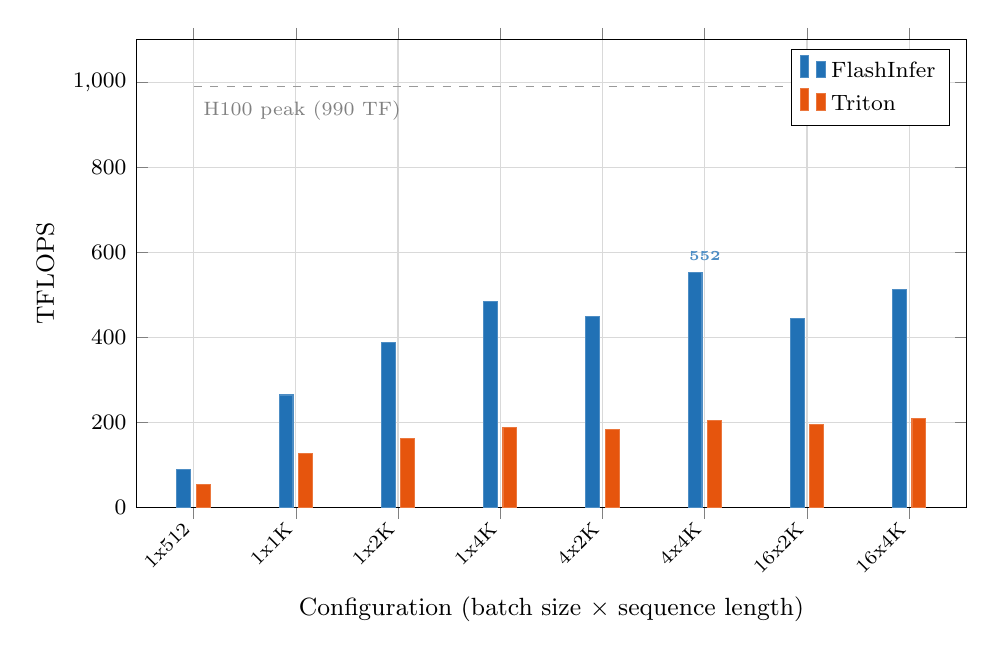
\begin{tikzpicture}
\begin{axis}[
  width=\columnwidth,
  height=0.62\columnwidth,
  ybar,
  bar width=5pt,
  xlabel={Configuration (batch size $\times$ sequence length)},
  ylabel={TFLOPS},
  symbolic x coords={1x512,1x1K,1x2K,1x4K,4x2K,4x4K,16x2K,16x4K},
  xtick=data,
  x tick label style={rotate=45, anchor=east, font=\scriptsize},
  ymin=0, ymax=1100,
  ytick={0,200,400,600,800,1000},
  grid=major, grid style={gray!30},
  enlarge x limits=0.08,
  clip=false,
]
% FlashInfer
\addplot[fill=fiblue, draw=fiblue!80] coordinates {
  (1x512,88) (1x1K,264) (1x2K,387) (1x4K,485)
  (4x2K,448) (4x4K,552) (16x2K,444) (16x4K,512)
};
% Triton
\addplot[fill=triorange, draw=triorange!80] coordinates {
  (1x512,54) (1x1K,126) (1x2K,161) (1x4K,188)
  (4x2K,183) (4x4K,204) (16x2K,195) (16x4K,209)
};
% H100 peak reference
\addplot[dashed, black!40, thin, forget plot, sharp plot]
  coordinates {(1x512,990) (16x4K,990)};
\node[font=\scriptsize, black!50, anchor=north west]
  at (axis cs:1x512,980) {H100 peak (990 TF)};
% Peak annotation
\node[font=\tiny, fiblue!80, anchor=south]
  at (axis cs:4x4K,558) {\textbf{552}};
\legend{FlashInfer, Triton}
\end{axis}
\end{tikzpicture}
\caption{Prefill compute throughput (Llama-3-8B GQA).  FlashInfer achieves 2.1--2.7$\times$ higher TFLOPS across all configurations, peaking at 552~TFLOPS (56\% of peak).  The gap widens with sequence length due to FlashInfer's TMA hardware loads and cooperative grid launch (Section~\ref{sec:prefill_ncu}).}
\label{fig:prefill_tflops}
\end{figure}

\subsection{Prefill: NCU Root Cause Analysis}
\label{sec:prefill_ncu}

\begin{table}[h]
\centering
\small
\caption{NCU metrics, prefill, bs=4, $S=2048$.}
\label{tab:ncu_prefill}
\begin{tabular}{@{}lcc@{}}
\toprule
Metric & FlashInfer & Triton \\
\midrule
Kernel       & \texttt{PrefillWith...} & \texttt{\_fwd\_kernel} \\
SM util.     & \textbf{52.0\%} & 32.7\% \\
DRAM util.   & 13.1\% & 9.3\% \\
Regs/thread  & 168 & \textbf{255} (max) \\
Active warps & 14.1\% & 12.5\% \\
Grid size    & 132 (cooperative) & 2048 \\
L1 global ld sectors & \textbf{108K} & 37.8M \\
L2 hit rate  & \textbf{86.4\%} & 72.0\% \\
Tensor insts & 2.23M & 2.23M \\
LOCAL mem (CUBIN) & \textbf{0 bytes} & \textbf{0 bytes} \\
Duration     & \textbf{368~$\mu$s} & 909~$\mu$s \\
\bottomrule
\end{tabular}
\end{table}

\subsubsection{Finding: TMA vs.\ Global Loads (Not ``Cache Hit Rate'')}
\label{sec:tma}

A naive reading of NCU's L1 sector counters (Table~\ref{tab:ncu_prefill}) yields: FlashInfer 97\% L1 hit rate, Triton 0.1\%.  \textbf{This is misleading.}

FlashInfer's Hopper kernel uses TMA (Tensor Memory Accelerator)~\cite{hopper}, a dedicated hardware unit that performs asynchronous bulk tensor copies directly from HBM/L2 into shared memory, \emph{bypassing the L1 global load data path entirely}.  The 108K L1 global load sectors are residual metadata accesses (indptr arrays, scalar parameters), not QKV tensor data.  The 37.8M sectors in Triton represent the \emph{actual} QKV working set flowing through L1 via standard \texttt{ld.global} instructions.

The correct comparison is at L2: FlashInfer achieves 86.4\% hit rate vs.\ Triton's 72.0\%.  FlashInfer's cooperative grid launch (132 blocks = 1 per SM) creates a controlled L2 working set; Triton's 2048-block grid generates 83\% more L2 misses (9.9M vs.\ 5.4M sectors) due to wave-quantization thrashing.

This distinction is architecturally fundamental.  TMA access is not ``better caching'' but a \emph{different hardware data path} unavailable to Triton's compiler, which generates standard \texttt{ld.global} PTX.

\subsubsection{Finding: No Register Spills (Occupancy-Only Bottleneck)}
\label{sec:spills}

Triton's prefill kernel compiles to 255 registers, the \texttt{sm\_90} hardware maximum.  A natural hypothesis is that registers spill to local memory, adding latency.  We tested this at three levels:

\begin{enumerate}[leftmargin=*,topsep=0pt]
  \item \textbf{NCU local memory counters}: The local memory wavefront counters (\texttt{l1tex..mem\_local\_op\_\allowbreak\{ld,st\}.sum}) returned \texttt{n/a} on all Hopper kernels (known NCU limitation on sm\_90).
  \item \textbf{PTX inspection}: Zero \texttt{.local} directives, zero \texttt{st.local} / \texttt{ld.local} instructions in the compiled PTX.
  \item \textbf{CUBIN resource dump} (\texttt{cuobjdump --dump-resource-usage}): \texttt{LOCAL:0} for \texttt{\_fwd\_kernel}.
\end{enumerate}

\textbf{Verdict}: Triton's 255-register kernel does \emph{not} spill.  The compiler fits all live variables within the register file at the cost of maximal register allocation.  The performance impact is purely occupancy: fewer warps per SM means fewer opportunities to hide memory latency.

Reducing Triton's register count (e.g., via different tiling or explicit \texttt{num\_stages} tuning) could improve occupancy and partially close the prefill gap, but the TMA access pattern difference (Section~\ref{sec:tma}) would remain.

\subsubsection{Finding: Cooperative Grid vs.\ Wave Quantization}

FlashInfer launches exactly 132 thread blocks (one per SM) using CUDA cooperative launch semantics.  This eliminates wave-quantization effects and enables persistent-kernel-style execution where each block processes multiple tiles sequentially with full shared memory and register file utilization.

Triton launches 2,048 blocks ($15.5\times$ more), dispatched in multiple waves.  Each wave evicts the previous wave's L2 residency, explaining the 14-point L2 hit rate gap (86.4\% vs.\ 72.0\%).

% ══════════════════════════════════════════════════════════════════════════════
\section{The MLA Reconstruction Bottleneck}
\label{sec:recon}

Having established confidence in our profiling infrastructure, we turn to our central question: how much of MLA's attention-layer time is spent on reconstruction?

Multi-head Latent Attention~\cite{deepseekv2} compresses KV cache to a low-rank latent $c_t \in \mathbb{R}^{d_\text{lora}}$ with $d_\text{lora}=512$.  During decode, full-dimensional K and V are \emph{reconstructed} via weight-absorbed batch matrix multiplications (BMMs):

\begin{align}
\text{BMM1:} \; & Q'_h = Q_h W^\text{kc}_h, \;\; W^\text{kc}_h \!\in\! \mathbb{R}^{d_\text{nope} \times d_\text{lora}} \nonumber \\
\text{BMM2:} \; & O_h = A_h W^\text{vc}_h, \;\; W^\text{vc}_h \!\in\! \mathbb{R}^{d_\text{lora} \times d_v} \nonumber
\end{align}

where $h = 1, \ldots, H$ heads.  These are batched GEMMs with batch dimension $H$, independent of KV sequence length.

\subsection{Cost Breakdown: DeepSeek-V3 Architecture}

We profile reconstruction BMMs separately from FlashInfer MLA attention on DeepSeek-V3-scale shapes ($H=128$, $d_\text{nope}=128$, $d_\text{lora}=512$, $d_v=128$).

\begin{table}[h]
\centering
\small
\caption{MLA reconstruction overhead per layer, DeepSeek-V3 shapes, $L_{kv}=2048$.  Reconstruction cost is independent of KV length.}
\label{tab:recon}
\begin{tabular}{@{}rrrrr@{}}
\toprule
BS & Recon ($\mu$s) & Attn ($\mu$s) & Recon \% & Model (ms) \\
\midrule
  1 & \textbf{35.6} &  23.0 & \textbf{60.7\%} & \textbf{2.17} \\
  4 & 35.4 &  27.2 & 56.6\% & 2.16 \\
 16 & 34.2 &  40.4 & 45.8\% & 2.08 \\
 64 & 34.1 &  83.6 & 29.0\% & 2.08 \\
128 & 38.4 & 154.4 & 19.9\% & 2.34 \\
256 & 66.9 & 293.6 & 18.6\% & 4.08 \\
512 & 109.4 & 584.5 & 15.8\% & 6.68 \\
\bottomrule
\end{tabular}
\end{table}

\textbf{Key finding:}  At batch size 1, reconstruction BMMs consume \textbf{60.7\%} of attention-layer time (35.6~$\mu$s vs.\ 23.0~$\mu$s for the attention kernel itself) (Table~\ref{tab:recon}, Figure~\ref{fig:recon_overhead}).  Across 61 layers, this totals \textbf{2.17~ms per token}, a fixed per-query overhead invisible to standard attention benchmarks.

\begin{figure}[t]
\centering
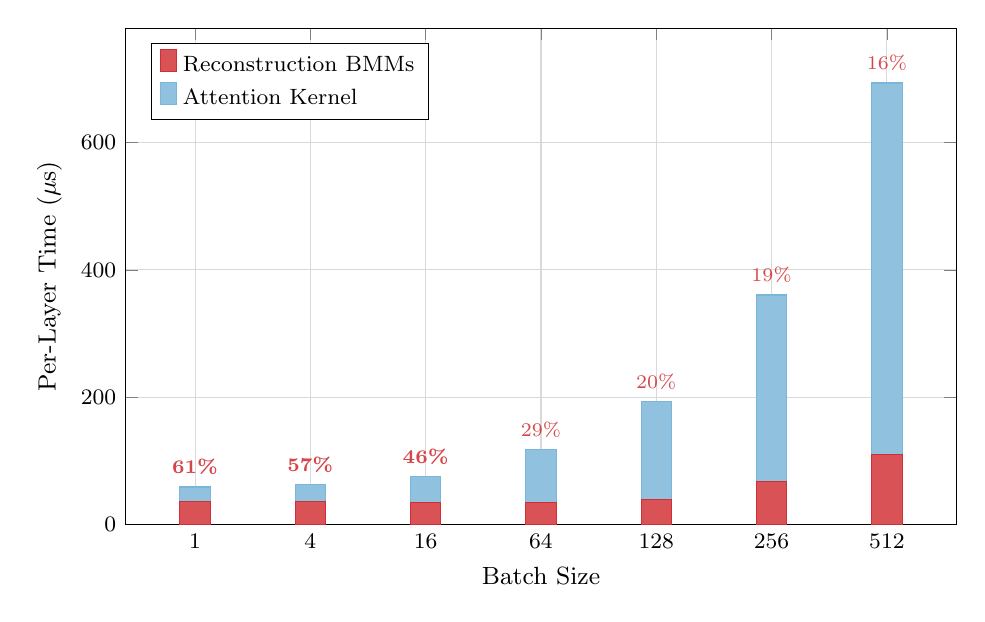
\begin{tikzpicture}
\begin{axis}[
  width=\columnwidth,
  height=0.65\columnwidth,
  ybar stacked,
  bar width=11pt,
  xlabel={Batch Size},
  ylabel={Per-Layer Time ($\mu$s)},
  symbolic x coords={1,4,16,64,128,256,512},
  xtick=data,
  ymin=0, ymax=780,
  grid=major, grid style={gray!30},
  enlarge x limits=0.1,
  clip=false,
  legend style={at={(0.03,0.97)}, anchor=north west},
]
% Reconstruction BMMs (bottom, red)
\addplot[fill=reconred!75, draw=reconred!90] coordinates {
  (1,35.6) (4,35.4) (16,34.2) (64,34.1) (128,38.4) (256,66.9) (512,109.4)
};
% Attention kernel (top, blue)
\addplot[fill=attnblue!75, draw=attnblue!90] coordinates {
  (1,23.0) (4,27.2) (16,40.4) (64,83.6) (128,154.4) (256,293.6) (512,584.5)
};
% Reconstruction % annotations above each bar
\node[font=\scriptsize\bfseries, reconred!80, anchor=south]
  at (axis cs:1,62) {61\%};
\node[font=\scriptsize\bfseries, reconred!80, anchor=south]
  at (axis cs:4,66) {57\%};
\node[font=\scriptsize\bfseries, reconred!80, anchor=south]
  at (axis cs:16,78) {46\%};
\node[font=\scriptsize, reconred!80, anchor=south]
  at (axis cs:64,121) {29\%};
\node[font=\scriptsize, reconred!80, anchor=south]
  at (axis cs:128,196) {20\%};
\node[font=\scriptsize, reconred!80, anchor=south]
  at (axis cs:256,364) {19\%};
\node[font=\scriptsize, reconred!80, anchor=south]
  at (axis cs:512,698) {16\%};
\legend{Reconstruction BMMs, Attention Kernel}
\end{axis}
\end{tikzpicture}
\caption{MLA attention-layer time decomposition per layer (DeepSeek-V3 shapes, $L_{kv}{=}2048$).  Reconstruction BMMs (red) dominate at small batch sizes (\textbf{61\% at bs=1}) and remain significant at bs=512.  Reconstruction cost is nearly constant (${\sim}$35~$\mu$s), independent of KV length; attention scales linearly.}
\label{fig:recon_overhead}
\end{figure}

\subsection{Roofline Analysis: Memory-Bound at All Batch Sizes}

\begin{table}[h]
\centering
\small
\caption{Arithmetic intensity and achieved bandwidth for reconstruction BMMs.  H100 roofline crossover: AI = 295 (990~TFLOPS / 3.35~TB/s).}
\label{tab:roofline}
\begin{tabular}{@{}rrrrr@{}}
\toprule
BS & AI (BMM1) & BW$_1$ & AI (BMM2) & BW$_2$ \\
\midrule
  1 & \textbf{0.97} &  954 & \textbf{0.97} &  952 \\
 16 & 15.5 & 1133 & 15.5 & 1137 \\
 64 & 62.1 & 1592 & 62.1 & 1607 \\
128 & \textbf{93.0} & \textbf{1837} & \textbf{93.0} & \textbf{2114} \\
256 & 93.0 & 1741 & 93.0 & 1770 \\
\bottomrule
\end{tabular}
\end{table}

Arithmetic intensity peaks at 93 (bs=128+), well below the crossover point of 295 (Table~\ref{tab:roofline}, Figure~\ref{fig:roofline}).  \textbf{All reconstruction BMMs are memory-bound.}  Achieved bandwidth ranges from 952~GB/s to 2,114~GB/s (28--63\% of HBM peak), leaving significant room for kernel optimization.

\textbf{Critical implication:}  Because reconstruction is memory-bound and weight-dominated (weight matrix is $128 \times 128 \times 512 \times 2 = 16$~MB per BMM, fixed regardless of batch size), reducing weight precision directly reduces the memory bandwidth bottleneck.

\begin{figure}[t]
\centering
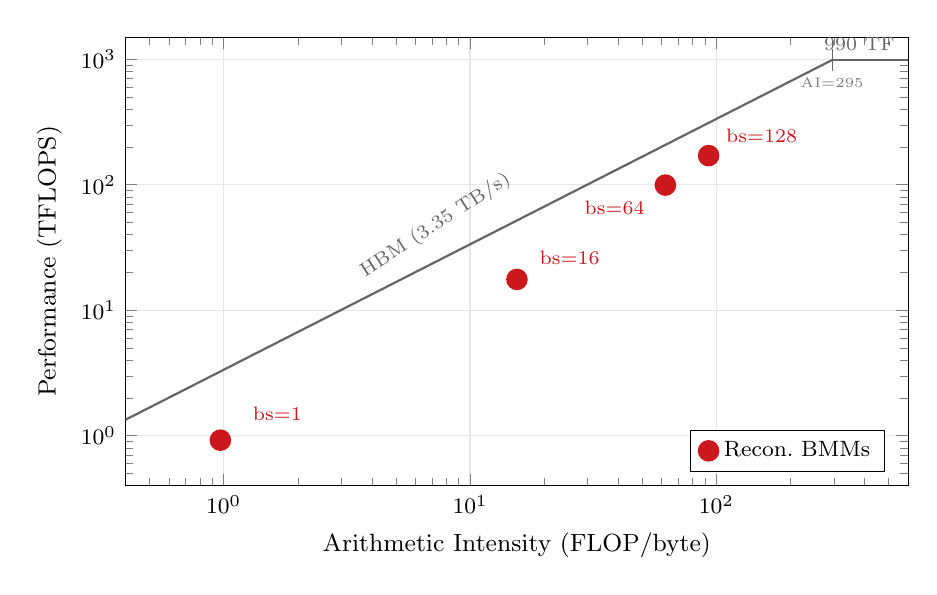
\begin{tikzpicture}
\begin{loglogaxis}[
  width=0.95\columnwidth,
  height=0.6\columnwidth,
  xlabel={Arithmetic Intensity (FLOP/byte)},
  ylabel={Performance (TFLOPS)},
  xmin=0.4, xmax=600,
  ymin=0.4, ymax=1500,
  grid=major, grid style={gray!20},
  clip=false,
  legend style={at={(0.97,0.03)}, anchor=south east},
]
% Memory ceiling: y = 3.35 * x
\addplot[thick, black!60, forget plot, domain=0.4:295, samples=2] {3.35*x};
% Compute ceiling: y = 989.4
\addplot[thick, black!60, forget plot, domain=295:600, samples=2] {989.4};
% Crossover marker
\addplot[only marks, mark=|, mark size=4, black!60, forget plot]
  coordinates {(295, 989.4)};
% Ceiling labels
\node[font=\scriptsize, black!60, rotate=33, anchor=south]
  at (axis cs:8,35) {HBM (3.35 TB/s)};
\node[font=\scriptsize, black!60, anchor=south east]
  at (axis cs:580,989.4) {990 TF};
\node[font=\tiny, black!50, anchor=north]
  at (axis cs:295,850) {AI=295};
% Reconstruction BMM data points
\addplot[only marks, mark=*, mark size=3.5, reconred, thick]
  coordinates {
    (0.97, 0.92) (15.5, 17.6) (62.1, 99.4) (93.0, 170.8)
  };
\addlegendentry{Recon.\ BMMs}
% Point labels
\node[font=\scriptsize, reconred, anchor=south west] at (axis cs:1.2,1.1) {bs=1};
\node[font=\scriptsize, reconred, anchor=south west] at (axis cs:17.5,19.5) {bs=16};
\node[font=\scriptsize, reconred, anchor=north east] at (axis cs:56,88) {bs=64};
\node[font=\scriptsize, reconred, anchor=south west] at (axis cs:100,182) {bs=128};
\end{loglogaxis}
\end{tikzpicture}
\caption{H100 roofline with MLA reconstruction BMMs.  All operating points fall on the memory-bound slope, well below the compute ceiling (crossover at AI=295).  Even at bs=128 (AI=93), reconstruction achieves only 55\% of the memory ceiling.}
\label{fig:roofline}
\end{figure}

% ══════════════════════════════════════════════════════════════════════════════
\section{INT4 Mitigation and the L2 Cache Barrier}
\label{sec:int4}

Reconstruction BMMs are memory-bound at all practical batch sizes, and their weight matrices dominate the data transfer.  Reducing weight precision should therefore yield proportional speedups.  We evaluate INT4 weight-only quantization of $W^\text{kc}$ and $W^\text{vc}$, addressing two questions: does it preserve quality, and does it deliver the expected performance gain?

\subsection{Perplexity Evaluation}

We evaluate on DeepSeek-V2-Lite (15.7B parameters) using wikitext-2 test set (308K tokens, stride-512 sliding window, max length 2048).  Three configurations:

\begin{table}[h]
\centering
\small
\caption{Wikitext-2 perplexity under INT4 quantization.  \texttt{kv\_b\_proj} is the reconstruction weight ($W^\text{kc}$/$W^\text{vc}$ combined).}
\label{tab:ppl}
\begin{tabular}{@{}lrrr@{}}
\toprule
Configuration & PPL & $\Delta$ & Weights quantized \\
\midrule
FP16 baseline       & \textbf{5.727} & ---    & 0 \\
INT4 selective       & 5.777 & \textbf{+0.051} & 27 (kv\_b\_proj) \\
INT4 all linear      & \textbf{11.784} & +6.057 & 5,209 \\
\bottomrule
\end{tabular}
\end{table}

\textbf{Selective INT4 quantization of reconstruction weights adds only +0.051 perplexity} (Table~\ref{tab:ppl}, Figure~\ref{fig:ppl}), an order of magnitude below the typical 0.5 quality threshold.  Naive INT4 of all linear weights, by contrast, more than doubles perplexity.

\begin{figure}[t]
\centering
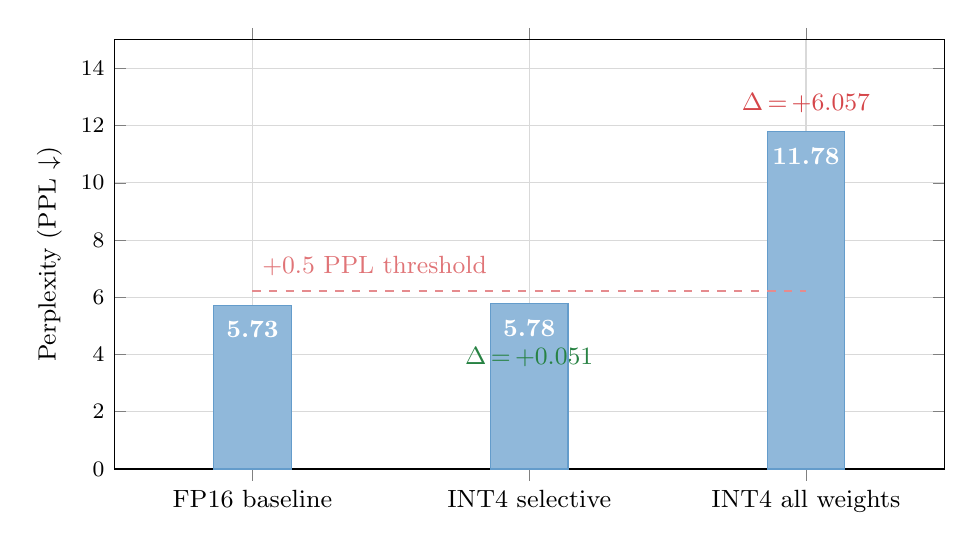
\begin{tikzpicture}
\begin{axis}[
  width=\columnwidth,
  height=0.58\columnwidth,
  ybar,
  bar width=28pt,
  ylabel={Perplexity (PPL $\downarrow$)},
  symbolic x coords={{FP16 baseline},{INT4 selective},{INT4 all weights}},
  xtick=data,
  x tick label style={font=\small, align=center, text width=2.4cm},
  ymin=0, ymax=15,
  ytick={0,2,4,6,8,10,12,14},
  grid=major, grid style={gray!30},
  enlarge x limits=0.25,
  clip=false,
]
\addplot[fill=fiblue!50, draw=fiblue!70] coordinates {
  ({FP16 baseline}, 5.727)
  ({INT4 selective}, 5.777)
  ({INT4 all weights}, 11.784)
};
% Quality threshold line (+0.5 from baseline)
\addplot[dashed, reconred!50, thick, forget plot, sharp plot]
  coordinates {({FP16 baseline},6.227) ({INT4 all weights},6.227)};
\node[font=\small, reconred!60, anchor=south west]
  at (axis cs:{FP16 baseline},6.4) {+0.5 PPL threshold};
% Value labels inside bars (white on blue)
\node[font=\small\bfseries, white, anchor=north]
  at (axis cs:{FP16 baseline},5.5) {5.73};
\node[font=\small\bfseries, white, anchor=north]
  at (axis cs:{INT4 selective},5.55) {5.78};
\node[font=\small\bfseries, white, anchor=north]
  at (axis cs:{INT4 all weights},11.55) {11.78};
% Delta annotations
\node[font=\small, predgreen!80!black, anchor=north]
  at (axis cs:{INT4 selective},4.6) {$\Delta$\,=\,+0.051};
\node[font=\small, reconred!80, anchor=south]
  at (axis cs:{INT4 all weights},12.1) {$\Delta$\,=\,+6.057};
\end{axis}
\end{tikzpicture}
\caption{Wikitext-2 perplexity under INT4 quantization (DeepSeek-V2-Lite).  Selective INT4 of reconstruction weights (\texttt{kv\_b\_proj}) adds only +0.051~PPL, well within the +0.5 quality threshold.  Naive INT4 of all linear weights severely degrades quality.}
\label{fig:ppl}
\end{figure}

\subsection{Why Reconstruction Weights Are Quantization-Friendly}

The $W^\text{kc}$ and $W^\text{vc}$ matrices are \emph{projection weights} that map between a compressed 512-dimensional latent space and 128-dimensional head spaces.  Several factors explain their quantization robustness:

\begin{enumerate}[leftmargin=*,topsep=0pt]
  \item \textbf{Low-rank structure}: The latent space was trained to be compressible; the projection matrices inherit smooth spectral properties.
  \item \textbf{Redundancy}: With $H=128$ heads each projecting from the same 512-dim latent, per-head reconstruction errors are averaged across heads before affecting output.
  \item \textbf{Post-softmax attenuation (hypothesized)}: BMM2 operates on attention-weighted values; quantization noise is attenuated by the softmax distribution's sparsity.
\end{enumerate}

\subsection{Theoretical Speedup}

For memory-bound operations, speedup from weight quantization equals the ratio of total data transferred:

\begin{equation}
\text{Speedup} = \frac{\text{Weight}_\text{FP16} + \text{Activation}_\text{FP16}}{\text{Weight}_\text{INT4} + \text{Scale/ZP} + \text{Activation}_\text{FP16}}
\label{eq:speedup}
\end{equation}

\begin{table}[h]
\centering
\small
\caption{Theoretical INT4 speedup for reconstruction BMMs.  Weight bytes dominate at small batch sizes.}
\label{tab:int4_speedup}
\begin{tabular}{@{}rrrrr@{}}
\toprule
BS & Wt (MB) & Act (MB) & INT4 eq.\ (MB) & Speedup \\
\midrule
  1 & 16.00 & 0.03 & 4.00 & \textbf{3.94$\times$} \\
  4 & 16.00 & 0.13 & 4.00 & 3.89$\times$ \\
 16 & 16.00 & 0.50 & 4.00 & 3.67$\times$ \\
 64 & 16.00 & 2.00 & 4.00 & 3.00$\times$ \\
128 & 16.00 & 4.00 & 4.00 & 2.50$\times$ \\
256 & 16.00 & 8.00 & 4.00 & 2.00$\times$ \\
\bottomrule
\end{tabular}
\end{table}

At batch size 1 (latency-critical single-query serving), the roofline predicts \textbf{3.94$\times$ speedup} (Table~\ref{tab:int4_speedup}), which would reduce the 2.17~ms full-model reconstruction overhead to $\sim$0.55~ms.

\subsection{Measured Kernel Performance}

We implemented a custom batched W4A16 Triton kernel that fuses the head dimension into the grid, avoiding 128 separate kernel launches.  The kernel dequantizes INT4 weights to FP16 in registers and uses tensor core \texttt{tl.dot} for the matmul.

\begin{table}[h]
\centering
\small
\caption{Measured INT4 kernel performance vs.\ cuBLAS FP16 \texttt{torch.bmm}.  ``FP16 loop'' = 128 individual \texttt{torch.mm} calls.}
\label{tab:int4_measured}
\begin{tabular}{@{}rrrrr@{}}
\toprule
BS & FP16 bmm & INT4 Tri & FP16 loop & Ratio \\
   & (ms) & (ms) & (ms) & INT4/FP16 \\
\midrule
  1 & \textbf{0.036} & 0.073 & 2.194 & \textbf{0.49$\times$} \\
  4 & 0.037 & 0.073 & 2.203 & 0.50$\times$ \\
 16 & 0.036 & 0.082 & 2.187 & 0.44$\times$ \\
 64 & 0.036 & 0.129 & 2.215 & 0.28$\times$ \\
128 & 0.040 & 0.187 & 2.211 & \textbf{0.21$\times$} \\
256 & 0.070 & 0.302 & 2.223 & 0.23$\times$ \\
\bottomrule
\end{tabular}
\end{table}

\textbf{The INT4 kernel is 2$\times$ slower than cuBLAS FP16, not 3.9$\times$ faster} (Table~\ref{tab:int4_measured}, Figure~\ref{fig:l2barrier}).  It is, however, 30$\times$ faster than a per-head FP16 loop (0.073~ms vs.\ 2.19~ms), confirming that the batched grid approach itself is effective.  The bottleneck is competing with cuBLAS, not the batching strategy.

\begin{figure}[t]
\centering
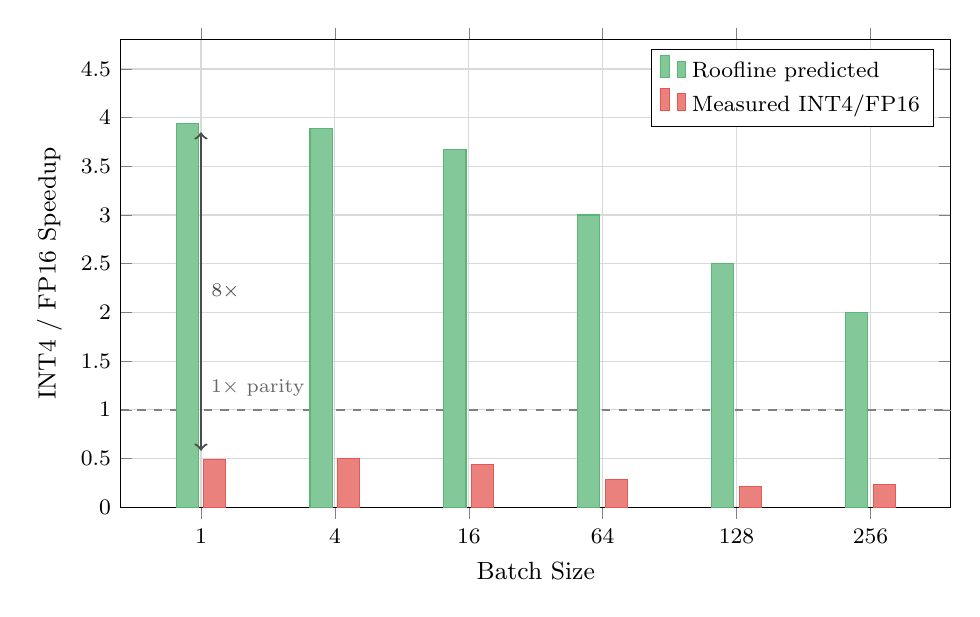
\begin{tikzpicture}
\begin{axis}[
  width=\columnwidth,
  height=0.62\columnwidth,
  ybar,
  bar width=8pt,
  xlabel={Batch Size},
  ylabel={INT4 / FP16 Speedup},
  symbolic x coords={1,4,16,64,128,256},
  xtick=data,
  ymin=0, ymax=4.8,
  ytick={0,0.5,1,1.5,2,2.5,3,3.5,4,4.5},
  grid=major, grid style={gray!30},
  enlarge x limits=0.12,
  clip=false,
  % 1x parity line
  extra y ticks={1.0},
  extra y tick labels={},
  extra y tick style={grid style={black!50, thick, dashed}},
]
% Roofline predicted
\addplot[fill=predgreen!60, draw=predgreen!80] coordinates {
  (1,3.94) (4,3.89) (16,3.67) (64,3.00) (128,2.50) (256,2.00)
};
% Measured
\addplot[fill=measred!60, draw=measred!80] coordinates {
  (1,0.49) (4,0.50) (16,0.44) (64,0.28) (128,0.21) (256,0.23)
};
% 1x parity label
\node[font=\scriptsize, black!60, anchor=south west]
  at (axis cs:1,1.04) {1$\times$ parity};
% Gap annotation for bs=1
\draw[<->, black!70, thick]
  (axis cs:1,0.58) -- (axis cs:1,3.85)
  node[midway, right, font=\scriptsize, black!70] {8$\times$};
\legend{Roofline predicted, Measured INT4/FP16}
\end{axis}
\end{tikzpicture}
\caption{The L2 cache barrier.  Roofline analysis predicts 2--3.9$\times$ INT4 speedup assuming HBM-bound operation.  Measured performance shows 0.2--0.5$\times$: the INT4 kernel is \emph{slower} than cuBLAS FP16.  The 16\,MB reconstruction weight fits in H100's 50\,MB L2; after first access, weights are served from L2 at ${\sim}$12\,TB/s, making HBM savings irrelevant.}
\label{fig:l2barrier}
\end{figure}

\subsection{The L2 Cache Barrier: Why Roofline Fails for Small-Matrix MLA Reconstruction}
\label{sec:l2barrier}

The 8$\times$ gap between roofline-predicted (3.9$\times$) and measured (0.49$\times$) performance has three contributing factors.  No single factor is sufficient: a fixed-shape rotation intervention (below) shows that removing factor~(1) alone still leaves INT4 at or below FP16 parity.

\textbf{(1) Partial L2 residency weakens the HBM-bound assumption.}  The standard roofline model~\cite{roofline} assumes data is served from HBM at 3.35~TB/s.  But the total reconstruction weight per BMM is $128 \times 128 \times 512 \times 2 = 16$~MB, within H100's 50~MB L2 cache.  Warm-loop counters (\texttt{ncu --cache-control none}, steady-state launch after 30 warm-ups) show \texttt{torch.bmm} re-reads only 4.0~MB of the 16.8~MB working set from DRAM per launch --- ${\sim}75\%$ L2-served --- at an effective serving bandwidth of 3.5--4.6~TB/s.  (The often-quoted ${\sim}12$~TB/s aggregate L2 bandwidth is not achieved by these kernels; CUDA-graph timing puts the incremental L2-era slope at 6.3~TB/s and total-bytes throughput at 3.5--4.6~TB/s.)  Reducing weight precision from FP16 to INT4 saves HBM bandwidth that \emph{was largely not the bottleneck}.

We validate the size dependence by scaling the weight matrix across the L2 boundary.  Holding $H{=}128$ and $d_\text{nope}{=}128$ fixed, we sweep $d_\text{lora}$ from 256 to 4096, producing FP16 weight sizes from 8~MB to 128~MB.  Figure~\ref{fig:l2sweep} shows the event-timed result: the INT4/FP16 time ratio drops from 1.91$\times$ at 8~MB to 1.08$\times$ at 128~MB.  Warm-state DRAM-read counters locate the actual residency cliff at \textbf{32--40~MB} (re-reads collapse to 2.2~MB at 32~MB weights, then snap to ${\sim}100\%$ of weight size at 40~MB and above): the \emph{effective} LRU residency capacity is ${\sim}36$~MB, below the nominal 50~MB, and the knee in Figure~\ref{fig:l2sweep} should be read against that corrected boundary.  Two confounds inflate the event-timed curve's flatness below 32~MB: a ${\sim}15.5~\mu$s per-launch timing floor (Section~2.4), and cuBLAS switching \texttt{nvjet} tile variants across the sweep.  CUDA-graph timing removes the floor and shows FP16 latency scaling smoothly at 6.3~TB/s below the cliff and 2.7~TB/s above it, with kernel-level INT4/FP16 ratios of 1.9$\times$ (16~MB) $\to$ 1.0--1.1$\times$ ($\geq$40~MB): \textbf{INT4 reaches parity above the cliff but never wins}.

\textbf{Weight-rotation intervention (residency removed at fixed shape).}  To test whether L2 residency is \emph{sufficient} to explain INT4's failure, we hold the MLA shape fixed (16~MB weights) and cycle each launch through $k$ independent weight copies inside a CUDA graph.  With $k{=}1$--$2$ (working set $\leq$32~MB, L2-resident) FP16 takes 4.8~$\mu$s per BMM; with $k{=}6$ (96~MB working set, residency destroyed) FP16 rises to 8.3~$\mu$s --- the +3.5~$\mu$s delta matching an HBM-rate weight reload.  INT4 is cache-state-insensitive (9.1 vs.\ 9.3~$\mu$s).  Critically, \textbf{INT4 remains 1.12$\times$ slower than FP16 even with FP16 forced to HBM}.  L2 residency accounts for the gap growing from 1.12$\times$ to 1.91$\times$, but eliminating it would not make this INT4 kernel win: the kernel runs 2.7$\times$ above its memory entitlement (${\sim}3.4~\mu$s for 4.2~MB at HBM rate) due to factor~(2).

\textbf{Controlled cache-residency intervention.}  To establish L2 residency as a causal factor rather than a correlate of matrix size, we hold the reconstruction shape fixed ($H{=}128$, $d_\text{nope}{=}128$, $d_\text{lora}{=}512$) and vary only the cache state immediately before each timed launch.  Under the warm condition, 20 untimed kernel executions load the 16\,MB weight tensor into L2 before measurement.  Under the cold condition, a memory sweep (4$\times$ L2 capacity: 256\,MB on H100, 192\,MB on A100) evicts L2 contents immediately before the timed launch, with explicit synchronization between eviction and measurement.

\begin{figure}[t]
\centering
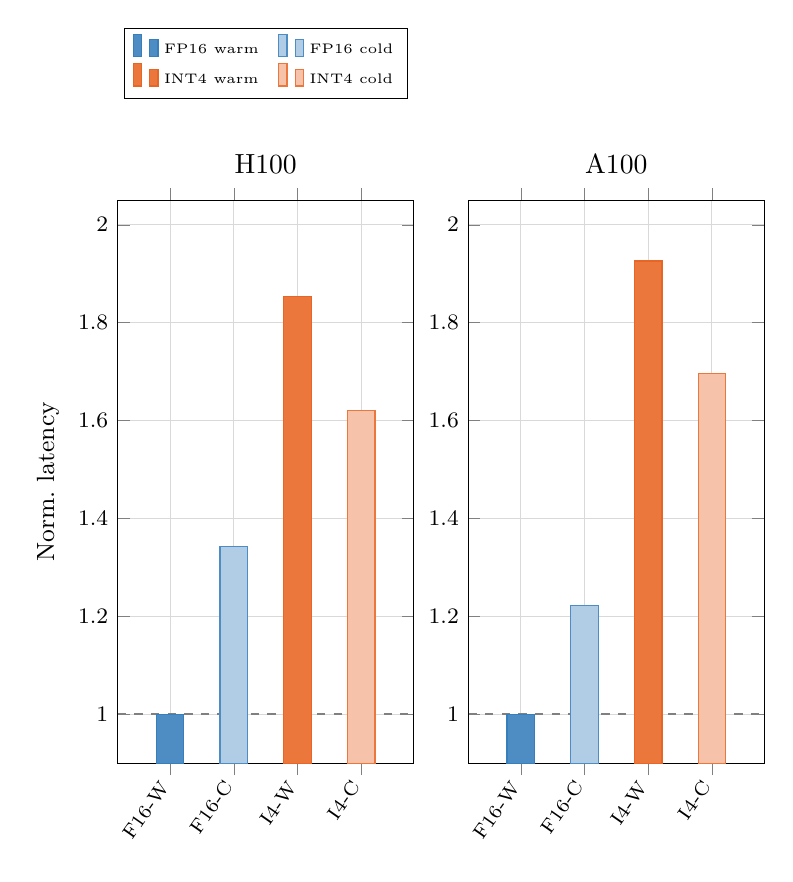
\begin{tikzpicture}
\begin{groupplot}[
  group style={group size=2 by 1, horizontal sep=0.7cm},
  width=0.44\columnwidth,
  height=0.72\columnwidth,
  ybar=10pt,
  ymin=0.9, ymax=2.05,
  ytick={1.0,1.2,1.4,1.6,1.8,2.0},
  grid=major, grid style={gray!30},
  xmin=0.5, xmax=4.5,
  xtick={1,2,3,4},
  xticklabels={F16-W,F16-C,I4-W,I4-C},
  x tick label style={rotate=55,anchor=east,font=\scriptsize},
  enlarge x limits=0.08,
  ylabel={Norm.\ latency},
  extra y ticks={1.0},
  extra y tick labels={},
  extra y tick style={grid style={black!50, thick, dashed}},
  legend style={font=\tiny, at={(0.5,1.18)}, anchor=south, legend columns=2, /tikz/every even column/.append style={column sep=5pt}},
]
\nextgroupplot[title={H100}]
\addplot[bar shift=0pt, fill=fiblue!80, draw=fiblue!90] coordinates {(1,1.000)};
\addplot[bar shift=0pt, fill=fiblue!35, draw=fiblue!80] coordinates {(2,1.343)};
\addplot[bar shift=0pt, fill=triorange!80, draw=triorange!90] coordinates {(3,1.853)};
\addplot[bar shift=0pt, fill=triorange!35, draw=triorange!80] coordinates {(4,1.621)};
\legend{FP16 warm, FP16 cold, INT4 warm, INT4 cold}

\nextgroupplot[title={A100}, ylabel={}]
\addplot[bar shift=0pt, fill=fiblue!80, draw=fiblue!90] coordinates {(1,1.000)};
\addplot[bar shift=0pt, fill=fiblue!35, draw=fiblue!80] coordinates {(2,1.222)};
\addplot[bar shift=0pt, fill=triorange!80, draw=triorange!90] coordinates {(3,1.926)};
\addplot[bar shift=0pt, fill=triorange!35, draw=triorange!80] coordinates {(4,1.697)};
\end{groupplot}
\end{tikzpicture}
\caption{Cache-residency intervention at fixed MLA reconstruction shape (BS=1, normalized to FP16-warm).  H100: eviction adds +4.8~$\mu$s to FP16 (= full 16~MB weight reload at HBM rate) and +3.9~$\mu$s to INT4, of which ${\sim}2.6~\mu$s is common-mode eviction overhead (expected INT4 reload: 1.3~$\mu$s).  The FP16 delta supports L2-residency dependence of the FP16 path; note that absolute deltas, not relative percentages, are the comparable quantity here since the two baselines differ ${\sim}2.6\times$.}
\label{fig:cache_intervention}
\end{figure}

Figure~\ref{fig:cache_intervention} shows this intervention on both H100 and A100.  We report \emph{absolute} latency deltas, since the FP16 and INT4 baselines differ by ${\sim}2.6\times$ and relative percentages are therefore not comparable across kernels.  On H100, forced eviction adds +4.8~$\mu$s to FP16 --- matching a full 16~MB weight reload at HBM rate (16~MB / 3.35~TB/s = 4.8~$\mu$s) --- and +3.9~$\mu$s to INT4.  INT4's expected reload is only ${\sim}1.3~\mu$s (4.2~MB packed), so roughly +2.6~$\mu$s of its delta is common-mode overhead from the eviction procedure itself (DRAM write-back of the dirty eviction buffer); a control with an 8~MB eviction buffer (too small to displace the weights) adds $<$0.3~$\mu$s to FP16, confirming the eviction buffer, not measurement noise, produces the common-mode term.  The FP16-specific component (+4.8~$\mu$s $\approx$ exact HBM reload time) supports L2-residency dependence of the FP16 path; an earlier version of this analysis reported the same data as relative percentages (FP16 +34\% vs.\ INT4 +17\%), which overstated the asymmetry.  NCU counter attribution per tensor allocation is not available in current tooling; the warm-loop \texttt{--cache-control none} DRAM-read counters and the rotation intervention above are the primary causal evidence, with this eviction experiment as corroboration.

\begin{figure}[t]
\centering
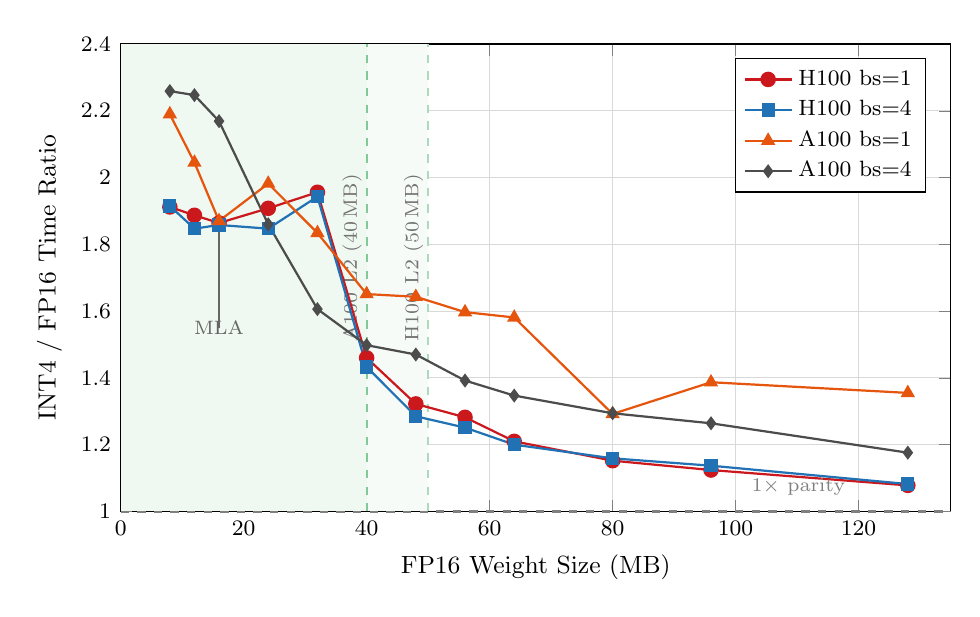
\begin{tikzpicture}
\begin{axis}[
  width=\columnwidth,
  height=0.62\columnwidth,
  xlabel={FP16 Weight Size (MB)},
  ylabel={INT4 / FP16 Time Ratio},
  xmin=0, xmax=135,
  ymin=1.0, ymax=2.4,
  ytick={1.0,1.2,1.4,1.6,1.8,2.0,2.2,2.4},
  grid=major, grid style={gray!30},
  clip=false,
  legend style={at={(0.97,0.97)}, anchor=north east},
  extra y ticks={1.0},
  extra y tick labels={},
  extra y tick style={grid style={black!50, thick, dashed}},
]
% L2 capacity regions
\fill[predgreen!8] (axis cs:0,1.0) rectangle (axis cs:40,2.4);
\fill[predgreen!4] (axis cs:40,1.0) rectangle (axis cs:50,2.4);
\draw[predgreen!60, thick, dashed] (axis cs:40,1.0) -- (axis cs:40,2.4);
\draw[predgreen!40, thick, dashed] (axis cs:50,1.0) -- (axis cs:50,2.4);
\node[font=\scriptsize, black!55, anchor=south, rotate=90] at (axis cs:40.8,1.76) {A100 L2 (40\,MB)};
\node[font=\scriptsize, black!55, anchor=south, rotate=90] at (axis cs:50.8,1.76) {H100 L2 (50\,MB)};
% H100 bs=1
\addplot[reconred, mark=*, mark size=2.4, thick] coordinates {
  (8,1.912) (12,1.887) (16,1.864) (24,1.908) (32,1.956)
  (40,1.460) (48,1.322) (56,1.282) (64,1.210) (80,1.152) (96,1.124) (128,1.078)
};
% H100 bs=4
\addplot[fiblue, mark=square*, mark size=2.0, thick] coordinates {
  (8,1.915) (12,1.847) (16,1.858) (24,1.847) (32,1.943)
  (40,1.433) (48,1.285) (56,1.251) (64,1.200) (80,1.159) (96,1.137) (128,1.082)
};
% A100 bs=1
\addplot[triorange, mark=triangle*, mark size=2.2, thick] coordinates {
  (8,2.190) (12,2.045) (16,1.870) (24,1.982) (32,1.834)
  (40,1.651) (48,1.643) (56,1.597) (64,1.581) (80,1.292) (96,1.387) (128,1.355)
};
% A100 bs=4
\addplot[black!70, mark=diamond*, mark size=1.9, thick] coordinates {
  (8,2.259) (12,2.247) (16,2.169) (24,1.860) (32,1.606)
  (40,1.498) (48,1.470) (56,1.392) (64,1.347) (80,1.294) (96,1.264) (128,1.176)
};
% 1x parity label
\node[font=\scriptsize, black!50, anchor=south west] at (axis cs:101,1.02) {1$\times$ parity};
% MLA operating point
\draw[->, black!60, thick] (axis cs:16,1.55) -- (axis cs:16,1.88);
\node[font=\scriptsize, black!60, anchor=south] at (axis cs:16,1.50) {MLA};
\legend{H100 bs=1, H100 bs=4, A100 bs=1, A100 bs=4}
\end{axis}
\end{tikzpicture}
\caption{Weight-size scaling on H100 and A100: event-timed INT4/FP16 ratio vs.\ FP16 weight size.  Below the knee INT4 is much slower; above it the ratio moves toward (but never below) parity as FP16 falls back to HBM.  Two caveats apply: (i) the H100 knee sits at 32--40\,MB, the \emph{effective} residency capacity measured by warm-state DRAM-read counters, not at the nominal 50\,MB; (ii) these event-timed curves embed a ${\sim}15.5\,\mu$s per-launch floor that flattens the small-size region --- CUDA-graph timing shows the same knee with kernel-level ratios of 1.9$\times$ $\to$ 1.0--1.1$\times$.  At MLA's 16\,MB operating point (arrow), both platforms are in the (partially) L2-resident regime.}
\label{fig:l2sweep}
\end{figure}

Replay-based NCU profiling across the same sweep classifies the two kernels --- with the caveat that these counters are \emph{cold-cache} (cache-flushed replay, Section~2.4) and therefore speak to kernel character, not to residency.  On H100, the FP16 cuBLAS kernel (\texttt{nvjet}, TMA-based) is memory-side at every size: SM utilization stays below 15\%, and DRAM utilization rises smoothly from 35\% at 8~MB to 83\% at 128~MB --- a duration-amortization effect (short kernels cannot sustain peak DRAM), \emph{not} an L2-boundary knee; the steepest rise occurs below 32~MB.  The INT4 Triton kernel is the opposite at every size: SM utilization scales from 33\% to 79\% (dequantization dominates) while DRAM utilization stays below 23\%.  On A100 the directions are the same (FP16 DRAM 43\%$\to$66\%, INT4 SM 51\%$\to$75\%).  There is thus no within-kernel memory-to-compute \emph{transition} anywhere in the sweep: FP16 is always memory-side and INT4 always dequant-compute-side; what changes with size is FP16's serving \emph{tier} (L2 below ${\sim}36$~MB effective capacity, HBM above), which is visible only in the warm-state counters and timing interventions above.  INT4 reads exactly 4$\times$ fewer DRAM bytes as expected, but converting that savings into latency requires the kernel to not be compute-bound, which it is.

This creates a paradox specific to MLA: the same low-rank compression that makes reconstruction weights small enough to be a latency concern \emph{also} makes them small enough to be L2-resident, defeating the primary motivation for weight quantization.  Standard LLM linear layers (e.g., FFN projections with weights in the hundreds of MB) do not exhibit this behavior.

\textbf{(2) INT4 dequantization shifts the bottleneck from memory to compute.}  The NCU data shows that the INT4 kernel is SM-bound (up to 79\% SM utilization) rather than DRAM-bound.  Bit masking, shifting, signed extension, and type conversion on every packed byte consume the freed bandwidth headroom.  Even when weights exceed L2 and FP16 falls back to HBM, INT4 cannot fully exploit its 4$\times$ data reduction because dequantization saturates the SMs first.

\textbf{(3) cuBLAS dispatch advantage.}  \texttt{torch.bmm} dispatches via the \texttt{nvjet} kernel family with TMA hardware loads (168 registers, L1 bypassed entirely), while our Triton kernel uses standard \texttt{ld.global} with 57 registers.  Under concurrent L2 contention, INT4 shows greater sensitivity to cache pressure than FP16---consistent with its irregular packed-byte access pattern.

\textbf{When does INT4 help?}  The L2 cache barrier is not absolute.  In production serving, concurrent operations (FFN GEMMs, attention across multiple layers, multi-tenant request batching) contend for L2 capacity and may evict reconstruction weights back to HBM.  However, our rotation intervention bounds what this can buy for the \emph{current} kernel: with FP16 fully evicted, this W4A16 implementation only reaches parity (1.12$\times$ slower at the 16~MB point; 1.0--1.1$\times$ across larger sizes).  Realizing an actual win under L2 pressure additionally requires a dequantization path that does not saturate the SMs --- e.g., INT8 tensor-core MMA with fused dequant --- after which fusing reconstruction across layers to exceed L2 capacity, or deploying on GPUs with smaller L2, would let the 4$\times$ byte reduction translate into latency.

\subsection{A Measured Cache-Aware Roofline}
\label{sec:carm}

The failures above are failures of the \emph{single-ceiling} roofline.  We therefore construct a cache-aware roofline in the spirit of Ilic et al.~\cite{carm}, with two extensions required for microsecond-scale LLM kernels, and with every parameter \emph{measured} on the target GPU (\texttt{measure\_carm\_params.py}) rather than taken from datasheets:

\begin{equation}
t \;=\; t_0 + \max\!\Big(\frac{B}{\mathrm{BW}(\mathrm{WS})},\; \frac{F}{P_\text{peak}}\Big),
\qquad
\mathrm{BW}(\mathrm{WS}) =
\begin{cases}
\mathrm{BW}_{L2}^{\text{eff}} & \mathrm{WS} < C_\text{eff}\\[2pt]
\mathrm{BW}_{\text{HBM}}^{\text{eff}} & \text{otherwise}
\end{cases}
\label{eq:carm}
\end{equation}

\textbf{Extension 1: capacity-gated bandwidth with effective parameters.}  The bandwidth ceiling is a function of working-set size, gated at the \emph{measured} effective residency capacity $C_\text{eff} \approx 36$~MB (not the nominal 50~MB), with measured tier bandwidths $\mathrm{BW}_{L2}^{\text{eff}} = 5.0$--$6.3$~TB/s (reduction- and GEMM-pattern, respectively; not the ${\sim}12$~TB/s aggregate figure) and $\mathrm{BW}_{\text{HBM}}^{\text{eff}} = 3.15$~TB/s.

\textbf{Extension 2: an explicit per-launch fixed cost} $t_0$ (measured: 2.8~$\mu$s graph-captured, 15.4~$\mu$s eager).  Classic rooflines plot performance against arithmetic intensity alone; for kernels whose data-path time is a few microseconds, $t_0$ dominates and every small-batch operating point sits far below the loft for reasons no bandwidth ceiling can express.  In Figure~\ref{fig:carm} (panel~A) we draw a per-point launch-floor cap $F/t_0$ that makes this regime explicit.

The INT4 kernel requires a different ceiling: it is bounded by dequantization throughput, not bandwidth.  Fitting $t = t_0' + W_\text{packed}\lceil \text{bs}/16\rceil / R_\text{dq}$ to the measured points gives $R_\text{dq} \approx 0.50$~TB/s of packed bytes, equivalent to an \emph{in-core ceiling of ${\sim}30$~TFLOPS --- 3\% of peak} --- which the INT4 operating points pin against at every batch size (Figure~\ref{fig:carm}, panel~A).  This single number explains the entire INT4 failure: no amount of bandwidth savings can help a kernel whose effective compute ceiling is 3\% of the machine.

The combined model predicts FP16 latency across batch sizes 1--512 with 10\% MAPE and INT4 with 18\% (Figure~\ref{fig:carm}, panel~C); the largest INT4 errors are at bs$\leq$16 where the single-M-tile dequant overlaps the fixed cost, making the model conservative.  Both the standard roofline's 3.9$\times$ INT4 prediction and the original ``L2 at 12~TB/s'' explanation are special cases of this model with wrong parameters: the former ignores $\mathrm{BW}(\mathrm{WS})$ and $R_\text{dq}$, the latter overestimates both tiers.

\begin{figure*}[t]
\centering
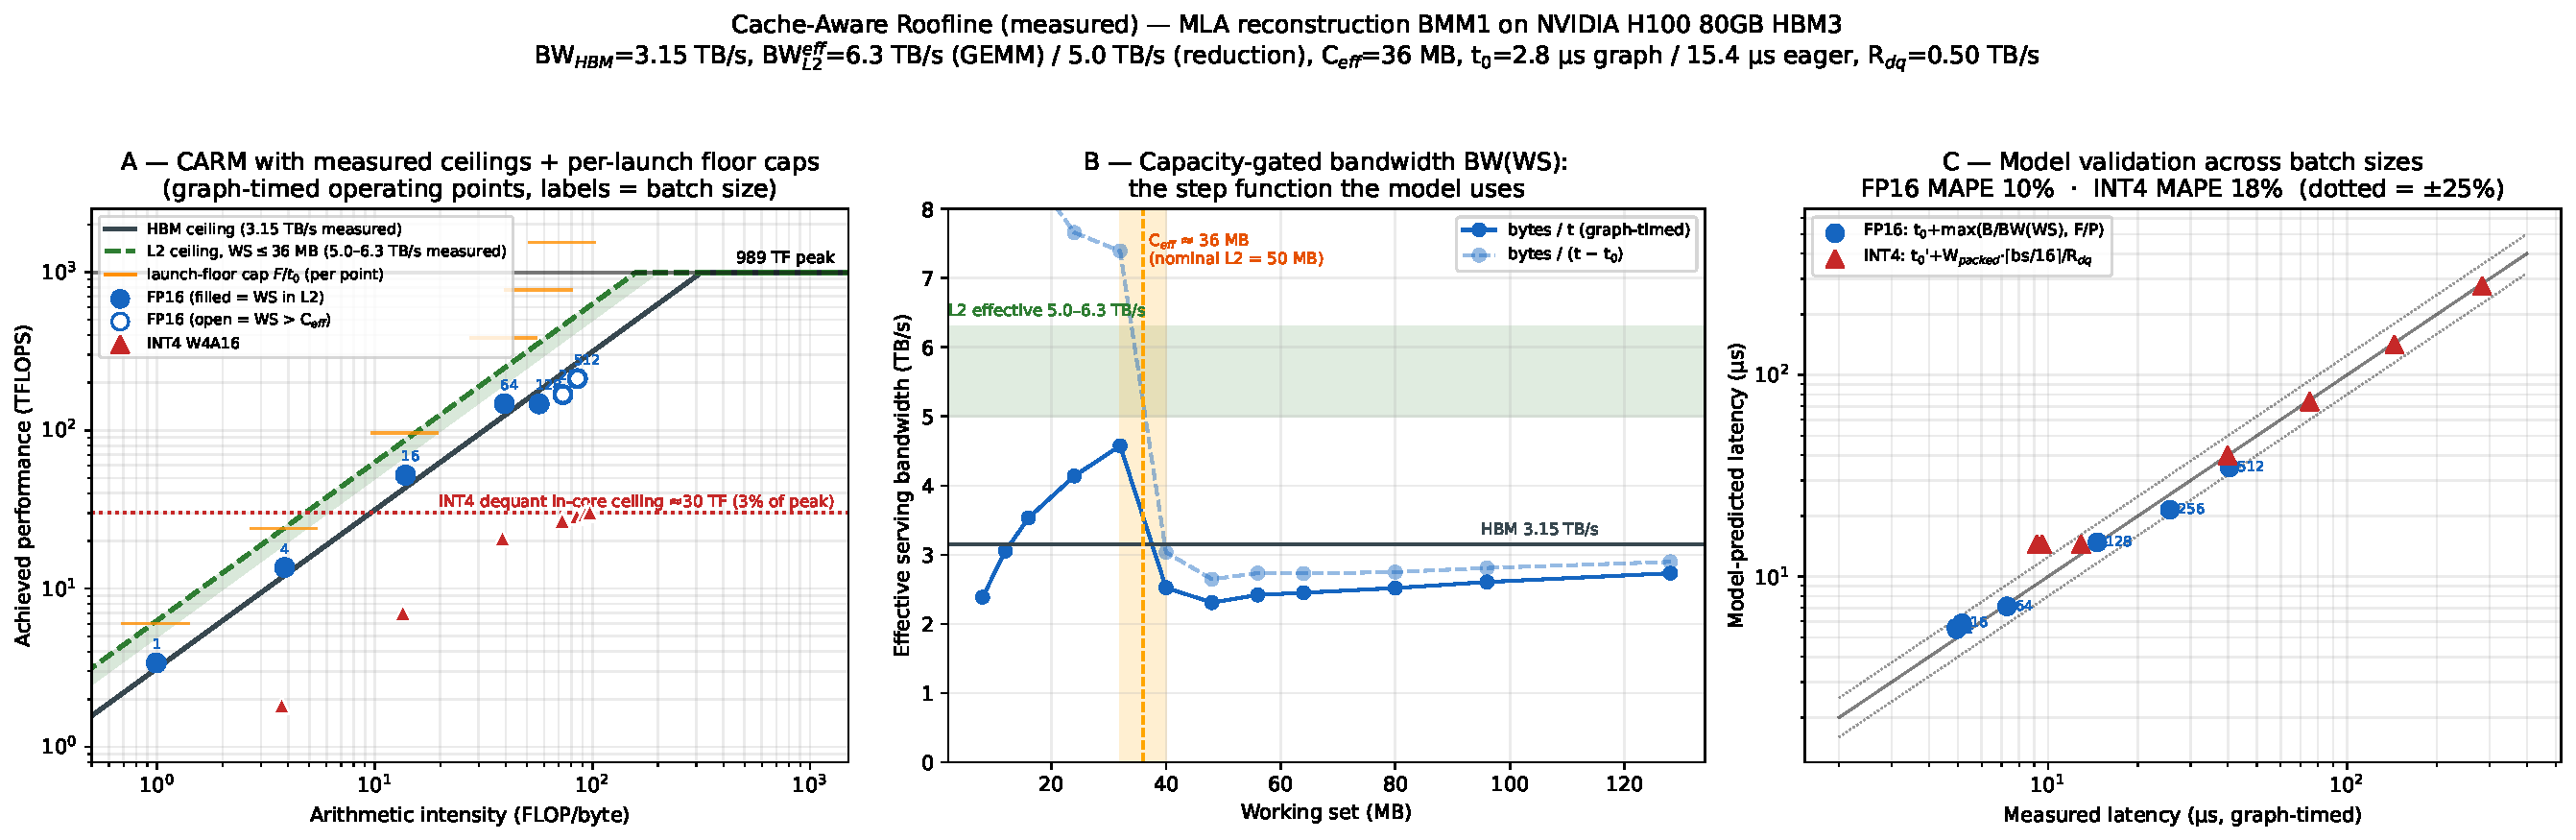
\includegraphics[width=\textwidth]{figures/carm_roofline.pdf}
\caption{Measured cache-aware roofline for MLA reconstruction (H100, graph-timed).  \textbf{A}: CARM with measured HBM and L2 ceilings, per-point launch-floor caps, and the fitted INT4 dequant in-core ceiling (${\sim}30$~TF); FP16 points (labeled by batch size) are filled when the working set fits $C_\text{eff}$.  \textbf{B}: the capacity-gated bandwidth function $\mathrm{BW}(\mathrm{WS})$ --- effective serving bandwidth vs.\ working set, with the measured residency cliff at 32--40~MB.  \textbf{C}: model validation, predicted vs.\ measured latency (dotted $= \pm 25\%$).}
\label{fig:carm}
\end{figure*}

% ══════════════════════════════════════════════════════════════════════════════
\section{End-to-End Context}
\label{sec:e2e}

To quantify the system-level impact of reconstruction, we contrast MLA against a standard GQA decode workload.

\begin{table}[h]
\centering
\small
\caption{Decode step decomposition, Qwen2.5-7B, bs=64.}
\label{tab:e2e}
\begin{tabular}{@{}lrr@{}}
\toprule
Component & Time ($\mu$s) & Share \\
\midrule
\textbf{Linear layers (GEMMs)} & \textbf{5,079} & \textbf{70.6\%} \\
Attention (FlashInfer) & 1,413 & 19.6\% \\
Norms (RMSNorm) & 145 & 2.0\% \\
Activation (SiLU) & 98 & 1.4\% \\
RoPE & 57 & 0.8\% \\
Other & 399 & 5.5\% \\
\bottomrule
\end{tabular}
\end{table}

Attention constitutes $\sim$20\% of decode time for GQA models (Table~\ref{tab:e2e}, Figure~\ref{fig:e2e}).  For MLA models like DeepSeek-V3, reconstruction overhead adds a further component: at bs=1, reconstruction GEMMs (2.17~ms across 61 layers) exceed the attention kernel cost (1.40~ms), making reconstruction the dominant attention-layer bottleneck.  Targeted optimization of reconstruction, whether through INT4 quantization or kernel fusion, is therefore higher-impact than further attention kernel tuning.

\begin{figure}[t]
\centering
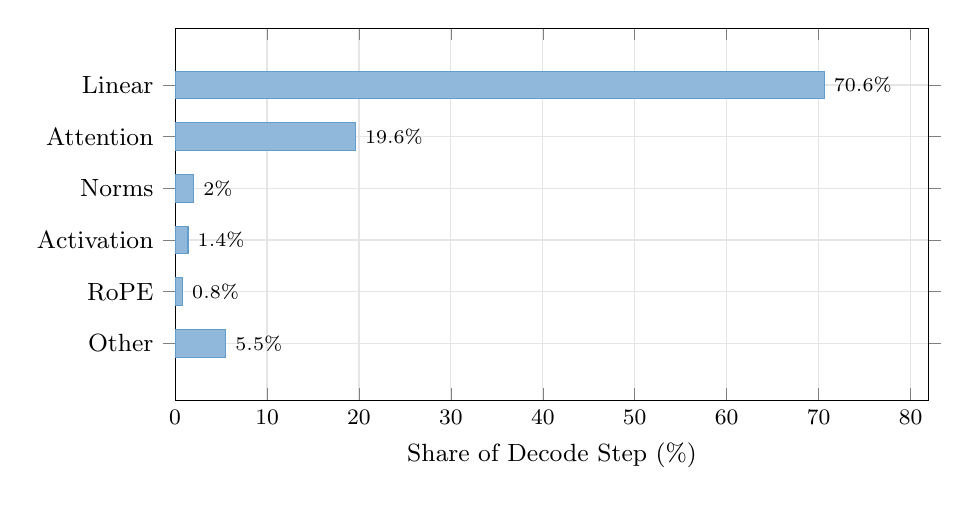
\begin{tikzpicture}
\begin{axis}[
  width=0.92\columnwidth,
  height=0.52\columnwidth,
  xbar,
  bar width=10pt,
  xlabel={Share of Decode Step (\%)},
  xmin=0, xmax=82,
  symbolic y coords={Other,RoPE,Activation,Norms,{Attention},{Linear}},
  ytick=data,
  y tick label style={font=\small},
  nodes near coords={\pgfmathprintnumber\pgfplotspointmeta\%},
  nodes near coords style={font=\scriptsize, anchor=west},
  grid=major, grid style={gray!20},
  enlarge y limits=0.22,
]
\addplot[fill=fiblue!50, draw=fiblue!70] coordinates {
  (70.6,{Linear})
  (19.6,{Attention})
  (2.0,Norms)
  (1.4,Activation)
  (0.8,RoPE)
  (5.5,Other)
};
\end{axis}
\end{tikzpicture}
\caption{Decode step decomposition (Qwen2.5-7B, bs=64).  Linear layers dominate at 71\%; attention is ${\sim}$20\%.  For MLA, reconstruction BMMs add to this: at bs=1, reconstruction (2.17\,ms) exceeds attention (1.40\,ms).}
\label{fig:e2e}
\end{figure}

% ══════════════════════════════════════════════════════════════════════════════
\section{Reproducibility}
\label{sec:repro}

\begin{table}[h]
\centering
\small
\caption{Reproducibility across 3 independent trials (warmup=20, iters=200).}
\label{tab:repro}
\begin{tabular}{@{}lcccr@{}}
\toprule
Config & T1 & T2 & T3 & CV \\
\midrule
FI dec bs=1   & 0.029 & 0.030 & 0.030 & 3.4\% \\
Tri dec bs=1  & 0.056 & 0.059 & 0.057 & 2.6\% \\
FI dec bs=64  & 0.187 & 0.187 & 0.187 & \textbf{$<$0.1\%} \\
Tri dec bs=64 & 0.216 & 0.216 & 0.216 & \textbf{$<$0.1\%} \\
FI dec bs=256 & 0.719 & 0.718 & 0.718 & \textbf{$<$0.1\%} \\
Tri dec bs=256& 0.813 & 0.813 & 0.813 & \textbf{$<$0.1\%} \\
\bottomrule
\end{tabular}
\end{table}

At bs$\geq$64, results are deterministic ($<$0.1\% CV) (Table~\ref{tab:repro}).  At bs=1, $\sim$3\% variance arises from GPU boost clock fluctuations on short ($\sim$28~$\mu$s) kernels.  Relative speedup ratios are stable across all trials.

% ══════════════════════════════════════════════════════════════════════════════
\section{Discussion}

Our analysis reveals a chain of findings: MLA's KV compression shifts the attention-layer bottleneck to reconstruction GEMMs (61\% at bs=1); these are memory-bound at all practical batch sizes; INT4 quantization preserves quality but fails to deliver speedup due to L2 cache residency.  We now discuss the implications.

\subsection{Implications for Compiler-Generated Attention}

The prefill gap is fundamental to the compiler architecture: Triton's MLIR$\to$PTX pipeline generates \texttt{ld.global} instructions because it has no TMA code generation path for attention patterns.  Triton 3.x introduced \texttt{tl.experimental\_descriptor\_load} for TMA access, but this requires manual descriptor setup that attention kernels have not adopted.  Closing the prefill gap requires either:

\begin{enumerate}[leftmargin=*,topsep=0pt]
  \item Triton compiler support for automatic TMA lowering of attention-shaped loads (research problem).
  \item Manual TMA integration in the Triton kernel source (engineering, loses portability).
  \item A higher-level DSL that targets both TMA and global load paths depending on the GPU architecture.
\end{enumerate}

The decode gap (1.1$\times$) is more tractable: Triton's two-phase split could be fused, and register tuning (\texttt{num\_warps}, tiling factors) could recover some bandwidth.

\subsection{The Occupancy Paradox as Design Principle}

FlashInfer's decode kernel shows that for memory-bound workloads, \emph{maximizing bandwidth per warp} outperforms \emph{maximizing warp count}.  At 183 registers, FlashInfer has 2.4$\times$ fewer active warps than Triton, yet extracts 10\% more HBM bandwidth.  This is consistent with the principle that memory-bound kernels benefit more from coalesced access patterns and prefetching than from raw occupancy~\cite{volkov2010}.

\subsection{MLA: Compression Shifts the Bottleneck}

MLA's 7.1$\times$ KV traffic reduction makes the attention kernel faster but creates a new bottleneck in the reconstruction GEMMs that were previously negligible.  At bs=1, reconstruction costs 61\% of attention-layer time.  This illustrates a general systems principle: optimizations that reduce data movement can shift workloads into regimes where cache hierarchy, rather than raw bandwidth, determines performance.  The implication for MLA specifically is that reconstruction overhead must be co-optimized with attention, not ignored.

\subsection{Selective Quantization: Quality Result}

Despite the kernel limitations, reconstruction weights tolerate quantization well: +0.051 PPL for selective INT4 vs.\ +6.057 for naive INT4 of all weights.  For future MLA serving systems, \textbf{reconstruction weights are the natural first target for aggressive quantization}, pending kernel support.

\subsection{Limitations}

\begin{itemize}[leftmargin=*,topsep=0pt]
  \item Single GPU; multi-GPU tensor-parallel workloads may show different ratios due to all-reduce overlap.
  \item GPU clocks not locked; absolute numbers carry $\sim$3\% uncertainty at small batch sizes.
  \item Per-launch CUDA-event timing carries a ${\sim}15.5~\mu$s floor; eager-mode bs$\leq$16 latencies (and the 61\% reconstruction share) are launch-overhead-inflated.  Serving engines that capture decode in CUDA graphs will see smaller absolute reconstruction overhead (graph-timed: ${\sim}4.8~\mu$s per BMM vs.\ ${\sim}17~\mu$s eager), though the recon-vs-attention ratio is less affected since both sides carry the floor.
  \item Replay-based NCU counters are cold-cache (\texttt{--cache-control all}); only the \texttt{--cache-control none} warm-loop counters and timing interventions speak to residency.
  \item INT4/FP16 ratios are software-stack-sensitive: PyTorch 2.9.1/Triton 3.5.1 yields 1.86$\times$ (16~MB) $\to$ 1.08$\times$ (128~MB) event-timed, while PyTorch 2.7/Triton 3.3 yields 2.75$\times$ $\to$ 1.58$\times$ on identical hardware.  Kernel-level (graph-timed) ratios are more stable (1.9$\times$ $\to$ 1.0--1.1$\times$).  Directional conclusions transfer; magnitudes do not.
  \item cuBLAS dispatches different \texttt{nvjet} tile variants across the weight-size sweep; the FP16 curve mixes kernel implementations.
  \item NCU local memory counters unavailable on Hopper (\texttt{n/a}); spill analysis relies on PTX/CUBIN inspection.
  \item INT4 kernel benchmarked in Triton only; a CUDA-native implementation with INT8 tensor cores may achieve different results.
  \item Perplexity evaluated on DeepSeek-V2-Lite (15.7B); larger models may show different quantization sensitivity.
  \item One model architecture per attention type.
\end{itemize}

% ══════════════════════════════════════════════════════════════════════════════
\section{Related Work}

\textbf{Attention kernels.}  FlashAttention~\cite{flashattention} and FlashAttention-2~\cite{flashattention2} introduced tiling-based exact attention with $O(N)$ memory.  FlashInfer~\cite{flashinfer} extends this with Hopper-native TMA support.  Triton~\cite{triton} enables Python-level GPU kernel development.  SGLang~\cite{sglang} integrates both backends for LLM serving.

\textbf{MLA architectures.}  DeepSeek-V2~\cite{deepseekv2} introduced Multi-head Latent Attention; DeepSeek-V3~\cite{deepseekv3} scaled it to 671B parameters with 128 attention heads.  While both papers describe the weight-absorbed reconstruction mechanism, neither quantifies its runtime cost relative to the attention kernel.

\textbf{Performance modeling.}  The roofline model~\cite{roofline} is the standard framework for reasoning about compute- vs.\ memory-bound kernels.  Ilic et al.~\cite{carm} extended it to cache-aware form with per-level bandwidth ceilings.  Our L2 cache barrier finding (Section~\ref{sec:l2barrier}) exposes a failure mode of single-level roofline analysis --- when working sets (partially) fit in L2, the effective bandwidth ceiling shifts from HBM toward L2 --- and Section~\ref{sec:carm} contributes a measured CARM variant with a capacity-gated ceiling, an explicit per-launch fixed cost, and a fitted dequantization in-core ceiling, validated to 10--18\% MAPE on the reconstruction kernels.  Volkov~\cite{volkov2010} showed that occupancy is not always the primary performance factor, motivating our analysis of FlashInfer's register-heavy approach.

\textbf{Weight quantization.}  GPTQ~\cite{gptq} and AWQ~\cite{awq} enable post-training INT4 weight quantization for LLM inference.  KVQuant~\cite{kvquant} applies quantization to the KV cache itself, targeting the memory footprint that MLA addresses architecturally.  QuaRot~\cite{quarot} uses rotation to eliminate outliers before 4-bit quantization.  All prior quantization work targets standard linear layers (FFN, attention projections), not the reconstruction matrices specific to MLA.  To our knowledge, no prior public work quantifies the reconstruction GEMM overhead in MLA or evaluates selective INT4 quantization of these weights.

% ══════════════════════════════════════════════════════════════════════════════
\section{Conclusion}

MLA's reconstruction GEMMs consume 61\% of eager-mode attention-layer time at batch size 1---a bottleneck that standard benchmarks miss, that single-level roofline analysis mispredicts by 8$\times$, and that naive INT4 quantization worsens rather than fixes.  We also provide a kernel-level characterization of FlashInfer vs.\ Triton attention on H100, identifying TMA hardware loads, memory access pattern quality, and cooperative grid launch as the three root causes of the performance gap.

The INT4 quantization results illustrate a subtlety in MLA optimization.  \textbf{Quality is safe}: selective INT4 adds only +0.051 perplexity.  \textbf{But speedup is not automatic}: our custom Triton W4A16 kernel achieves 0.49$\times$ of cuBLAS FP16 through two stacked mechanisms --- ${\sim}75\%$ of the 16~MB reconstruction weights are L2-served in steady state (effective capacity ${\sim}36$~MB, effective bandwidth 3.5--4.6~TB/s), removing most of the HBM savings INT4 targets; and the dequantization-bound kernel forfeits the remainder, losing to FP16 even when residency is experimentally removed.  The gap between roofline-predicted (3.9$\times$) and realized performance is specific to small, (partially) L2-resident weight matrices, a regime common in MLA but absent from standard LLM linear layers.  Closing this gap requires CUDA-native INT8 tensor core kernels (fixing the dequant path) \emph{and} either cross-layer weight fusion beyond L2 capacity or deployment under L2 pressure --- fixing residency alone is provably insufficient for this kernel.

All profiling scripts, raw data, and the perplexity evaluation code are publicly available for reproduction.

% ══════════════════════════════════════════════════════════════════════════════

\bibliographystyle{plain}
\bibliography{references}

\end{document}
